\documentclass{beamer}

% --------
% Packages
% --------

%encoding
%--------------------------------------
\usepackage[T1]{fontenc}
\usepackage[utf8]{inputenc}
%--------------------------------------
%Portuguese-specific commands
%--------------------------------------
\usepackage[portuguese]{babel}
%--------------------------------------
%Hyphenation rules
%--------------------------------------
\usepackage{hyphenat}
\hyphenation{mate-mática recu-perar}
%--------------------------------------
%encoding
%--------------------------------------
\usepackage[T1]{fontenc}
\usepackage[utf8]{inputenc}
%--------------------------------------
%Portuguese-specific commands
%--------------------------------------
\usepackage[portuguese]{babel}
%--------------------------------------
%Hyphenation rules
%--------------------------------------
\usepackage{hyphenat}
\hyphenation{mate-mática recu-perar}

%--------------------------------------
% Math
%--------------------------------------
\usepackage{amsmath}
\usepackage{amssymb}
\usepackage{amsfonts}
\usepackage{amsthm}

\theoremstyle{definition}
\newtheorem{defn}{Definição}[section]
\newtheorem{conj}{Conjecture}[section]
\newtheorem{exmp}{Example}[section]

%--------------------------------------
% Extra
%--------------------------------------
\usepackage{array}

\usepackage{graphicx}
\graphicspath{{images/}}

%--------------------------------------
% Diagrams
%--------------------------------------
\usepackage{tikz}
\usetikzlibrary{positioning}

\tikzset{basic/.style={draw,fill=blue!20,text width=1em,text badly centered}}
\tikzset{input/.style={basic,circle}}
\tikzset{output/.style={basic,circle}}
\tikzset{weights/.style={basic,rectangle}}
\tikzset{functions/.style={basic,circle,fill=blue!10}}

%--------------------------------------
% New Commands
%--------------------------------------
\newcommand{\exptd}[1]{\mathbf{E}\left[#1\right]}
\newcommand{\vt}[1]{\boldsymbol{#1}}
\newcommand{\trans}[1]{{#1}^\intercal}
\newcommand{\norm}[1]{\lvert#1\rvert}
\newcommand{\cov}[2]{\textbf{cov}\left(#1,\, #2\right)}

%--------------------------------------
% Beamer Colors
%--------------------------------------
\definecolor{background}{RGB}{204,243,255}
\setbeamercolor{block title}{bg=blue!30}
\setbeamercolor{block body}{bg=background}

\usetheme{metropolis}
\title{LEVI \- Inteligência Artificial}
\subtitle{A modern beamer theme}
\date{\today}
\author{Marcos Benevides}

\institute{Universidade Federal do Maranhão}

\begin{document}
\maketitle

\begin{frame}{Table of contents}
  \setbeamertemplate{section in toc}[sections numbered]
  \tableofcontents%[hideallsubsections]
\end{frame}

\section{Análise de componentes principais}

\begin{frame}{Variância}
  \begin{figure}[t]
    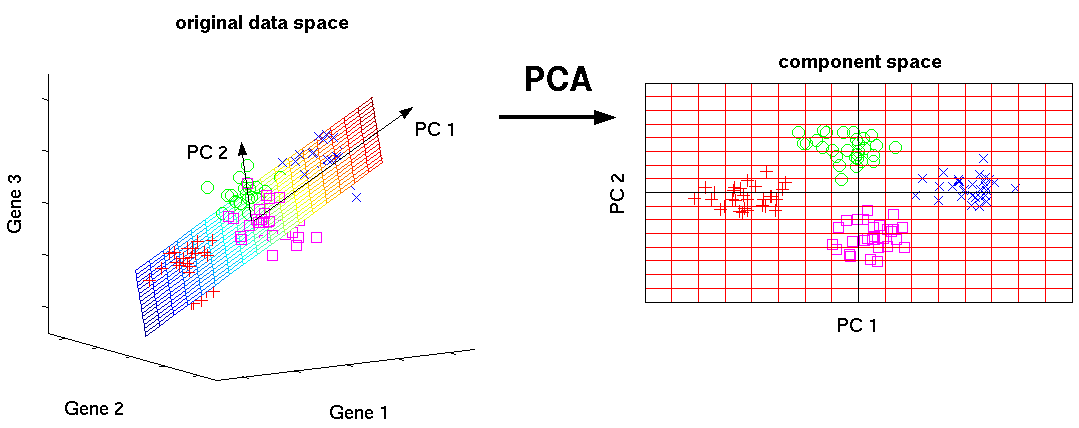
\includegraphics[width=\textwidth]{pca.png}
    \caption{Fonte: \cite{scholz2006approaches}}
    \centering
  \end{figure}
\end{frame}

\begin{frame}{Problema}

  \begin{table}
    \centering
    \begin{tabular}{ |c|c|c|c|c|c| }
    \hline
    & $x_1$ & $x_2$ & $\cdots$ & $x_{n-1}$ & $x_{n}$ \\ 
    \hline
    1 & & & & & \\ 
    \hline
    2 & & & & & \\ 
    \hline
    $\vdots$ & & & & & \\ 
    \hline
    m & & & & & \\ 
    \hline
    \end{tabular}
    \caption{Tabela com $n$ características e $m$ observações}
  \end{table}

  \begin{itemize}
    \item Como escolher os componentes (características) mais importantes?
  \end{itemize}

\end{frame}

\begin{frame}{Variância}
  \[ \sigma^2 = \frac{1}{n-1} \vt{x} \trans{\vt{x}} \]
  onde $n = \norm{\vt{x}}$.
\end{frame}

\begin{frame}{Covariância}
  \begin{defn}{Variáveis aleatórias em vetores coluna:}
    \[ \cov{x}{y} = \exptd{(\vt{x} - \exptd{\vt{x}}) \trans{(\vt{y} - \exptd{\vt{y}})}} \]

    \begin{align*}
      \cov{x}{x} &= \exptd{(\vt{x} - \exptd{\vt{x}}) \trans{(\vt{x} - \exptd{\vt{x}})}}\\
      &= \exptd{\vt{x} \trans{\vt{x}}}
    \end{align*}
  \end{defn}
\end{frame}

\begin{frame}{Covariância}

\end{frame}

\section{Perceptron}

\begin{frame}{O Modelo de McCullogh e Pitts}

  \begin{figure}[t]
    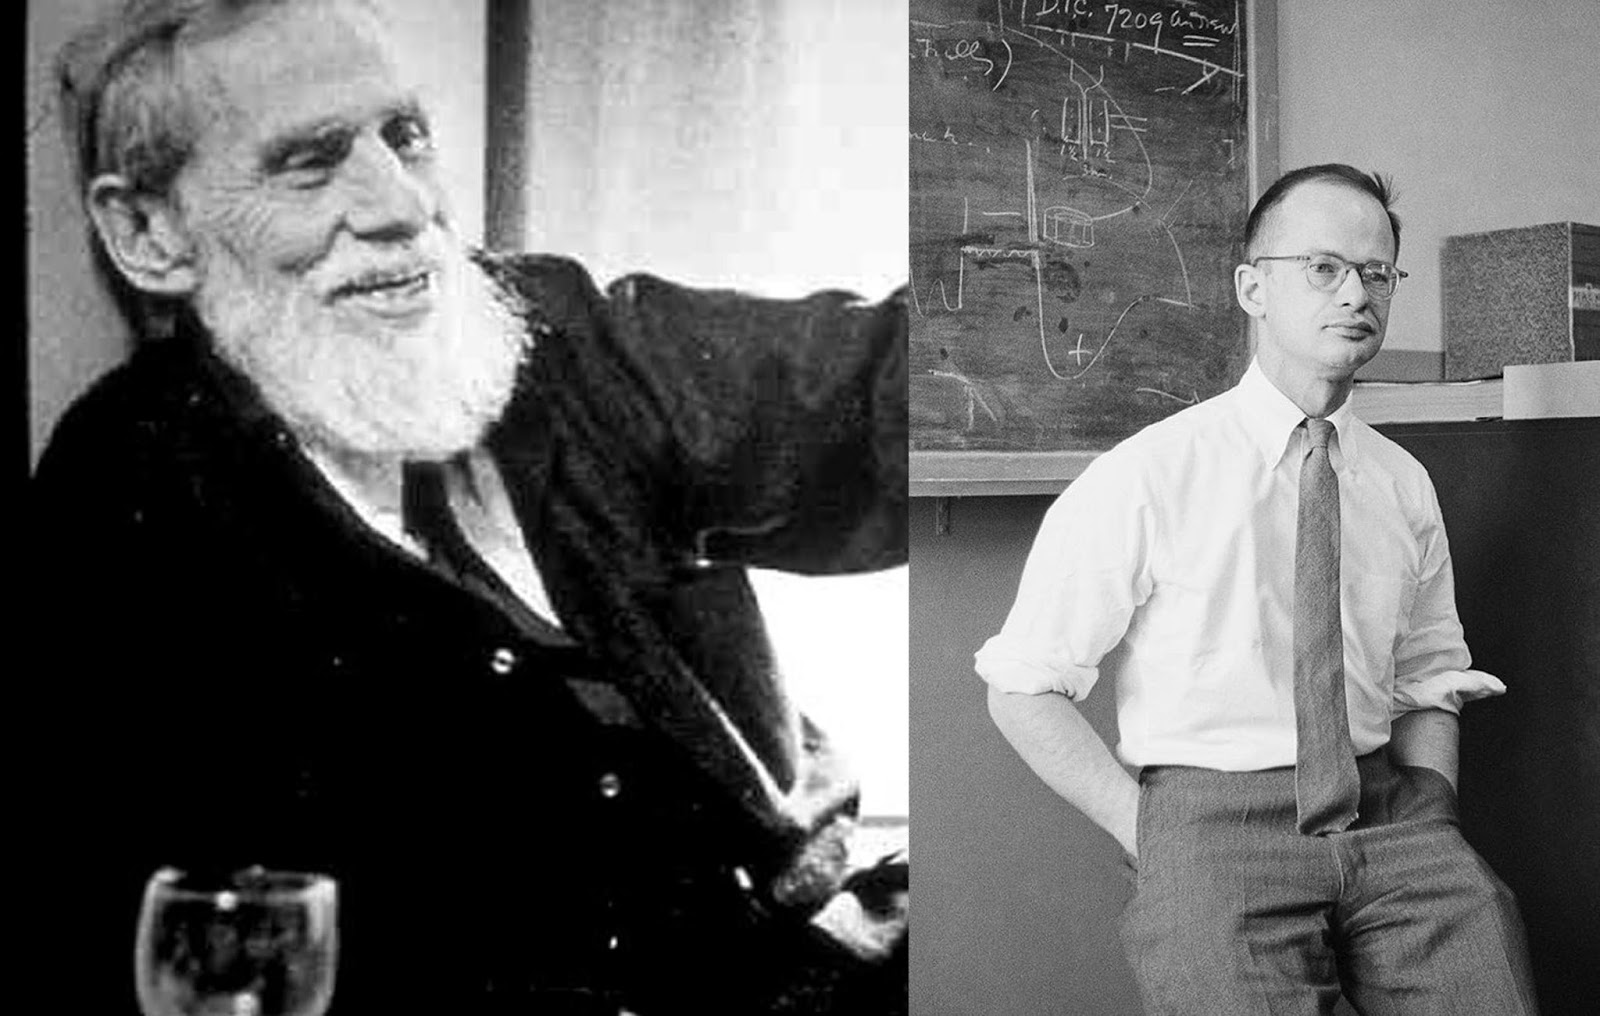
\includegraphics[width=0.8\textwidth]{warren_pitts.jpeg}
    \centering
  \end{figure}

\end{frame}

\begin{frame}{O Modelo de McCullogh e Pitts}

  \begin{figure}[t]
    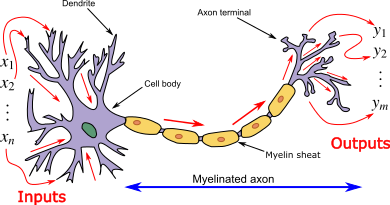
\includegraphics[width=0.8\textwidth]{neuron3.png}
    \caption{Neurônio biológico}
    \centering
  \end{figure}

\end{frame}

\begin{frame}{O Modelo de McCullogh e Pitts}

  \begin{figure}[t]
    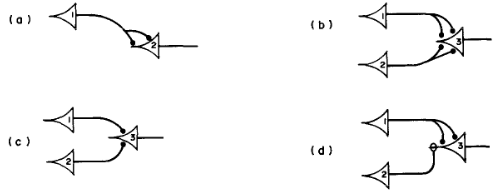
\includegraphics[width=\textwidth]{neuron1.png}
    \caption{Fonte: \cite{mcculloch1943logical}}
    \centering
  \end{figure}

\end{frame}

\begin{frame}{Aprendizado de Hebb}

  Quando um neurônio $x_i$ repetidamente ativa um neurônio $y$ a
  conexão entre $x_i$ e $y$ fica mais forte:

  \[ w_{i} = w_{i} + \eta x_i y \]

  \pause

  \begin{itemize}
    \item Conexões fortes apenas se reforçam (os pesos nunca se reduzem).
    \item Não existe noção de \"competição\" ou de limites pro aprendizado.
  \end{itemize}

\end{frame}

\begin{frame}{Aprendizado de Hebb (Generalizado)}

  \[ w_{ij} = w_{ij} + \eta y_j \left(x_i - \sum_{k=1}^{j} w_{ik}y_{k} \right)\]

  Um input é distribuido de forma incremental nos múltiplos outputs.

\end{frame}

\begin{frame}{Perceptron - Rosenblatt}

  \begin{figure}
    \begin{tikzpicture}
      \node[functions] (center) {};
      \node[below of=center,font=\scriptsize,text width=4em] (threshold) {Limiar (T)};
      \draw[thick] (0.5em,0.5em) -- (0,0.5em) -- (0,-0.5em) -- (-0.5em,-0.5em);
      \node[output, right=1.5em of center] (Y) {Y};
      \draw (0em,0.75em) -- (0em,-0.75em);
      \draw (0.75em,0em) -- (-0.75em,0em);
      \node[right of=center] (right) {};
        \path[draw,->] (center) -- (right);
      \node[functions,left=3em of center] (left) {$\sum$};
        \path[draw,->] (left) -- (center);
      \node[weights,left=3em of left] (2) {$w_2$} -- (2) node[input,left of=2] (l2) {$x_2$};
        \path[draw,->] (l2) -- (2);
        \path[draw,->] (2) -- (left);
      \node[below of=2] (dots) {$\vdots$} -- (dots) node[left of=dots] (ldots) {$\vdots$};
      \node[weights,below of=dots] (n) {$w_n$} -- (n) node[input,left of=n] (ln) {$x_n$};
        \path[draw,->] (ln) -- (n);
        \path[draw,->] (n) -- (left);
      \node[weights,above of=2] (1) {$w_1$} -- (1) node[input,left of=1] (l1) {$x_1$};
        \path[draw,->] (l1) -- (1);
        \path[draw,->] (1) -- (left);
      \node[weights,above of=1] (0) {$w_0$} -- (0) node[input,left of=0] (l0) {$x_0$};
        \path[draw,->] (l0) -- (0);
        \path[draw,->] (0) -- (left);
      \node[below of=ln,font=\scriptsize] {Inputs};
      \node[below of=n,font=\scriptsize] {Pesos};
    \end{tikzpicture}
  \centering
  \end{figure}

\begin{align}
Y = \left\{
  \begin{array}{cc}
    1 & \text{ se } \sum_{i} w_i x_i - T > 0 \\
    0 & \text{ caso contrário } \\
  \end{array} \right.
\end{align}

\end{frame}

%encoding
%--------------------------------------

{\setbeamercolor{palette primary}{fg=black, bg=yellow}
\begin{frame}[standout]
  Perguntas?
\end{frame}
}

\begin{frame}{Créditos:}

  Baseado nos materiais de:
  \begin{itemize}
    \item \href{http://deeplearning.cs.cmu.edu/}{http://deeplearning.cs.cmu.edu}
  \end{itemize}

\end{frame}


\begin{frame}[allowframebreaks]{Referências}

  \bibliography{references}
  \bibliographystyle{apalike}

\end{frame}

\end{document}
